% Chapter Template

\chapter{Approaches} % Main chapter title

\label{ch:03} % Change X to a consecutive number; for referencing this chapter elsewhere, use \ref{ChapterX}


The normal inference task can be simply stated as follows:

Given a structured point cloud $ V^{W\times H\times 3} $,
We would like to estimate the normal map  $ N^{W\times H \times 3} $, where each normal  $ \textbf{n}^{3\times 1} $ at point $ \textbf{v}^{3\times 1} \in N $ is a unit vector with its direction point outward of the surface and perpendicular to the tangent plane of the surface at point $ \textbf{p}^{3\times 1} $.

In this chapter, we first introduced an optimization based method using singular value decomposition (SVD). Then, we introduced the main work of this thesis, a deep learning based method which use gated convolution layers for normal inference. 

\section{Neighbor based surface normal estimation}
\subsection{Approach}

The idea behind the neighbor based method is to fit a plane $ \Pi $ using the $ k $ neighbors $ \textbf{p}_1, ..., \textbf{p}_k \in \mathbb{R}^3 $ of the point $ \textbf{p} $, calculate the normal  $ \tilde{\textbf{n}} $ of the plane. Then the actual normal $ \textbf{n} \approx \tilde{\textbf{n}}  $.

It is under the assumption that the point and its neighbors are located in the same plane. This is usually not hold for the most of the surface, but if $ k $ in a suitable scale and point cloud is dense enough, it is enough to get a good result. As shown in Figure \ref{fig:svd-normal}. 

Specifically, it is not necessary to find the exact plane equation to solve the normal. Instead, the normal can be derived based on an equation system (\ref{eq:normal-overdetermined-equation}). The normal $ \tilde{\textbf{n}} $ of plane $ \Pi $ is perpendicular to all the vector on the plane $ \Pi $, we can construct $ k $ vectors on plane $ \Pi $ use point $ \textbf{p} $ and its $ k $ neighbors $ \textbf{p}_1, ..., \textbf{p}_k \in \mathbb{R}^3 $ , which are assumed on the same plane, therefore we can a set of vector $ \textbf{v}_1, ..., \textbf{v}_k \in \mathbb{R}^3 $ and each of them satisfied $ \textbf{v}_i \cdot \tilde{\textbf{n}} = 0$. Then, the equation system can be constructed as 
\begin{equation}{\label{eq:normal-overdetermined-equation}}
	A \cdot \textbf{n} = 0
\end{equation}
where $ A \in \mathbb{R}^{k\times 3} $ is the vector matrix vertically stacked by $ \textbf{v}_1, ..., \textbf{v}_k $.
In order to avoid trivial solution, one more constraint should be added
\[ \|  \bn_{3 \times 1} \|_2^2 = 1  \]
which also let the normal to be a unit vector.

To calculate a valid normal, at least 3 points are required, i.e. $ k>=3 $. For the sake of robust, more points can be used to reduce the measuring error. For the case $ k>3 $, the equation system is usually over-determined, then the equation system mentioned above can be converted to follow optimization problem
\begin{equation}
	\begin{array}{rrclcl}
		\displaystyle \min & \multicolumn{3}{l}{\| A  \bn \|^2} \\
		\\
		\textrm{s.t.} & \| \bn \|^2 & = & 1 
	\end{array}
\end{equation}
which can be solved by singular value decomposition(SVD). Let the decomposition of 
\[ A=U\Sigma V^T \]
The solution i.e. normal is the last column of $ V $.


At last, all the normals should point ot view point $ \textbf{s} $, thus the direction of a normal should be inverted if 
\begin{equation}\label{eq:normal-invertion}
	\textbf{n} \cdot (\textbf{p}  - \textbf{s}) > 0
\end{equation}

Repeat the procedure for all the points in the point cloud to get the entire normal map. 

\subsection{Evaluation}
The neighbor based method can predict the normal map in a good way when the given point cloud is dense, as shown in Figure \ref{fig:svd-normal}. It can successfully predict the smooth surface of the dragon object, especially the flakes and the tails of the dragon. 

However, it failed in the areas such as hindleg, horn and the mouth, which consists mainly by sharp edges. This is because the neighbors points in these area do not hold the assumption of coplanarity, the normals of these neighbors can be very different. 
\begin{figure}[th]
	\centering
	\includegraphics[width=.25\textwidth]{./Figures/svd-synthetic/no-noise/fancy_eval_2_groundtruth.png}
	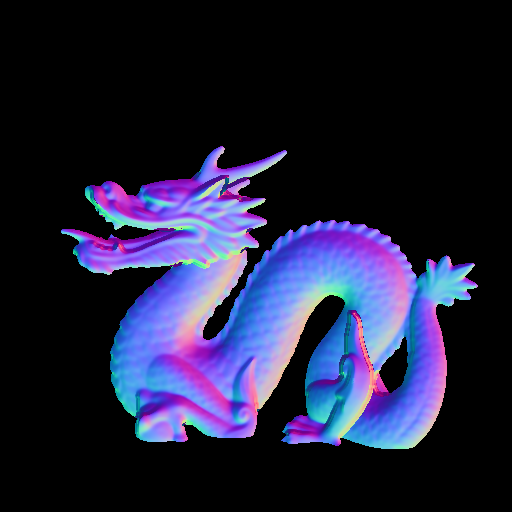
\includegraphics[width=.25\textwidth]{./Figures/svd-synthetic/no-noise/fancy_eval_2_normal_SVD.png}
	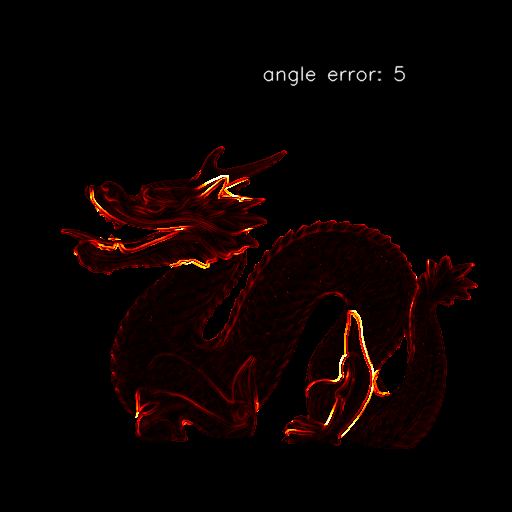
\includegraphics[width=.25\textwidth]{./Figures/svd-synthetic/no-noise/fancy_eval_2_error_SVD.png}
	
	\label{fig:svd-normal}
	\caption{Normal map of a dragon object predicted by neighbor based method. k=2, angle error=5 \textbf{Left}: ground-truth normal map \textbf{Middle}: predicted normal map, \textbf{Right}: Error map}
\end{figure}
The neighbor based method is depended on a well-chosen parameter $ k $. Figure \ref{fig:svd-k-eval} shows the evaluation on different $ k $ values. When $ k=1 $, the average error of the whole image is the lowest one, most of the normals are close to the ground-truth but the outline edges, which are the areas that surface normal changed extremely sever. For the case $ k=2 $, the sharp edges are more smooth and cause more error, like the eyes area of the dragon. Compare to the first case, the outline edge error goes better. Most of the edge errors are reduced when $ k=2 $, since more neighbor points join the evaluation and it reduces the effect of outliers. However, for the area of horn outline, hindleg outline, the error goes worse. In this case, most of the neighbors of these points are outliers and thus failed this approach.  $ k=3 $ and $ k=4 $ further increase the angle errors in $ k=2 $.
\begin{figure}[th]
	\centering
	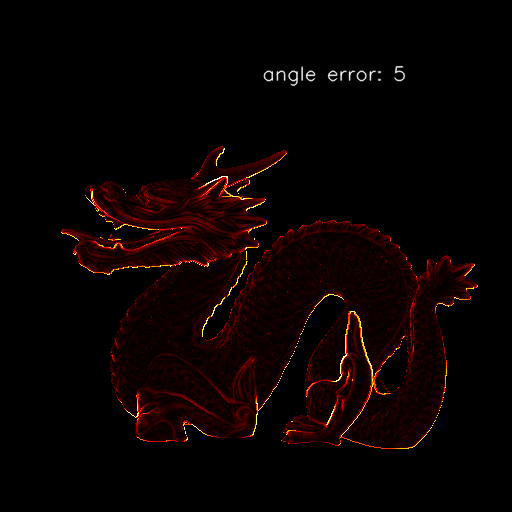
\includegraphics[width=.2\textwidth]{./Figures/svd-synthetic/k-compare/k1.png}
	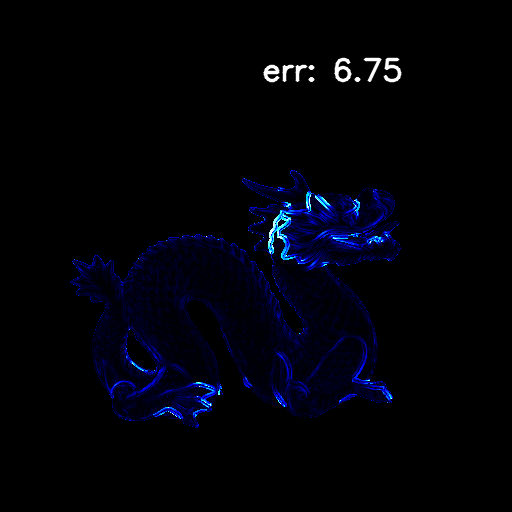
\includegraphics[width=.2\textwidth]{./Figures/svd-synthetic/k-compare/k2.png}
	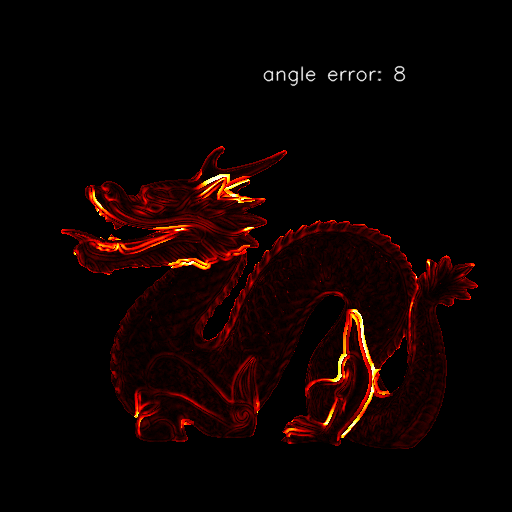
\includegraphics[width=.2\textwidth]{./Figures/svd-synthetic/k-compare/k3.png}
	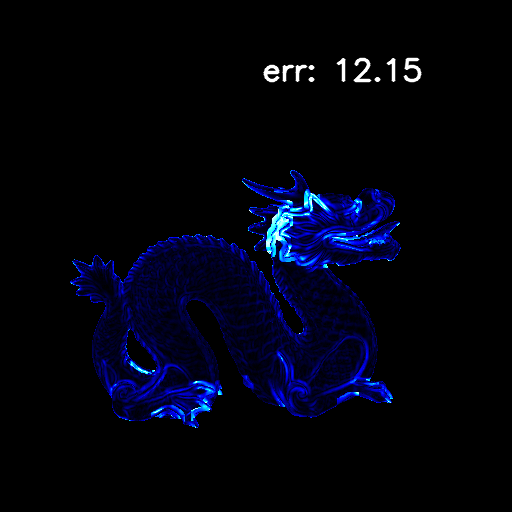
\includegraphics[width=.2\textwidth]{./Figures/svd-synthetic/k-compare/k4.png}	
	\label{fig:svd-k-eval}
	\caption{Error map of neighbor based method with different $ k $ values. From left to right, $ k=1,2,3,4 $ separately.}
\end{figure}

The performance of neighbor based method is good enough for a well chosen $ k $, and it can be further improved by simply use different $ k $ for different area prediction. However, for the case of noised point cloud as input, the approach will broken, since the noise will failed the neighbor selection and also reduce the number of possible neighbors of each point for a fixed $ k $.
\begin{figure}[th]
	\centering
	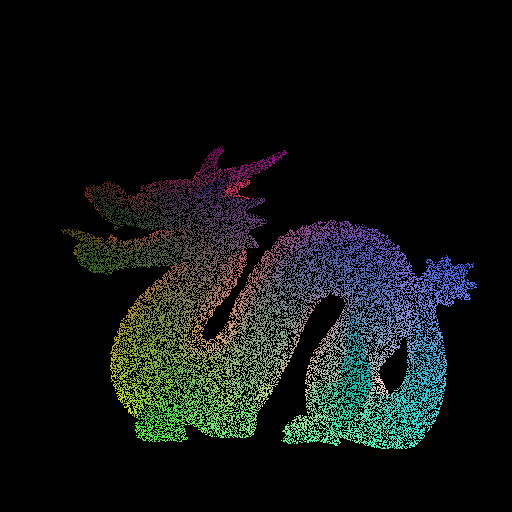
\includegraphics[width=.2\textwidth]{./Figures/svd-synthetic/noise/fancy_eval_2_point_cloud_noise.png}
	\includegraphics[width=.2\textwidth]{./Figures/svd-synthetic/noise/fancy_eval_2_groundtruth.png}
	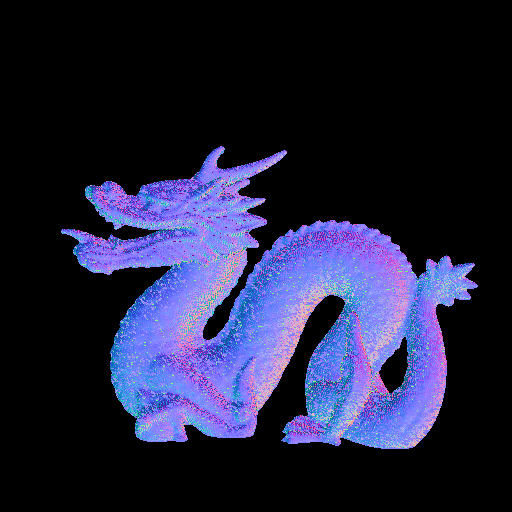
\includegraphics[width=.2\textwidth]{./Figures/svd-synthetic/noise/fancy_eval_2_normal_SVD.png}
	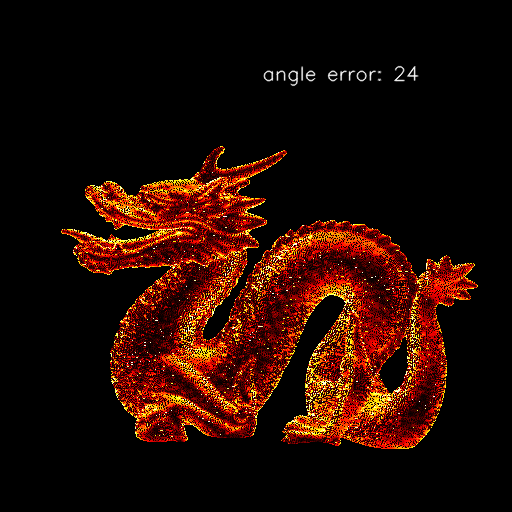
\includegraphics[width=.2\textwidth]{./Figures/svd-synthetic/noise/fancy_eval_2_error_SVD.png}	
	\label{fig:svd-noise}
	\caption{Evaluation of neighbor based method on a noised dragon model}
\end{figure}






% ---------------------- gated convolution neural network ------------------------
\section{Gated Convolution neural network for surface normal estimation}
\label{gcnn}


Recently, deep learning based method achieved a great succeed for image processing. ( \cite{yolov3}, \cite{efficientDet}) These network architectures use a batch of RGB / Grayscale images as input and are employed for classification problems. Usually, the images are convoluted with a convolution layer and downsampling with pooling layers. The outputs of the network consist of a single value to represent the index of the corresponding class (\cite{efficientDet}) or with a set of values to represent the position of bounding boxes.(\cite{yolov3}). However, in many other vision tasks, like normal map inference, the output is demanded as the same shape as the input. Instead of predicting one or several classes for the whole input matrix, the class for each pixel requires for prediction. In this case, the traditional network architecture is not suitable anymore.

%% upsampling 
It is worth to noticed that, the output of normal inference CNN model is not one or several labels but an entire image or normal map with same size. 
%% talk about image upsampling, unet
Recently,\cite{unet} proposed an architecture called UNet for biomedical image segmentations. The architecture is shown in Figure \ref{fig:u-net}.The first half network is a usual classification convolutional network, the second half replace the pooling layers and traditional fc layers in the traditional CNNs to upsampling layers, thus in the end of the second half, the output is able to back to the input size. The proposed network can successfully assigned each pixel a class for segmentation tasks. Under this symmetric network, an input image is downsampled 4 times and upsampled 4 times. Output image has exactly the same size as input image. The downsampling and upsampling both have large number of feature channels, which guarantee the network propagates the information to higher resolution layers.

\begin{figure}[th]
	\centering
	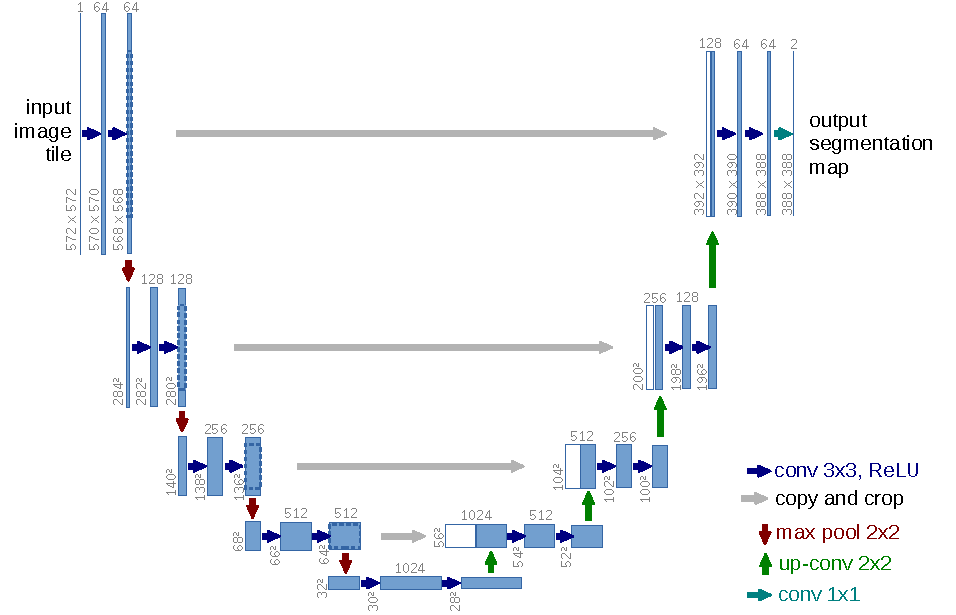
\includegraphics[width=.8\textwidth]{./Figures/u-net-illustration-correct-scale2.pdf}
	\label{fig:u-net}
	\caption{The structure of UNet. \cite{unet}}
\end{figure}


The UNet is based on standard convolution layers to construct the network. This is reasonable for image processing task with full-dense input, since no missing pixels exist. 
However, for the input of noised point cloud, the valid and invalid pixels will be treated equally if we still perform standard convolution layers. Since the aim of the network is not learning the pattern of noise, but the noise with eternally changing patterns will confuse the network, and it fails the normal inference, a mask is required to distinguish two kinds of pixels. 

% why we need a mask
\cite{pncnn0} use binary mask to indicate valid pixels, and further use normalized convolution to predict the output. The normalized convolution is shown as follows

\begin{equation}
	\begin{array}{rrclcl}
		O(x,y) = 
		\begin{cases}
			\dfrac{\Sigma_i^k\Sigma_j^k W(i,j) \cdot I(x-i,y-j) \cdot M(x-i,y-j)}{\Sigma_i^k\Sigma_j^k W(i,j) \cdot M(x-i,y-j)}, & \text{if}\ \sum_{i}^k\sum_{j}^k M(i,j)>0 \\
			0, & \text{otherwise}
		\end{cases}
	\end{array}
\end{equation}

where $ k $ is the kernel size, $ (x,y) $ is the position in input, $ (i,j) $ is the displacement in kenel, $ M $ is the corresponding mask. A binary mask uses 1 to indicate valid pixels and 0 otherwise. $ \odot $ denotes element-wise multiplication.

Normalized convolution layer added the weight to the mask. However, a initialization for the mask is still required, and the propagation of the mask remain a tricky task. 

\subsection{Gated Convolution}

% introduce gconv
\cite{gated_activation} proposed a gated activation unit to model more complex interactions comparing to standard CNN layers, which mainly inspired by the multiplicative units exist in Long Short-Term Memory proposed by \cite{lstm} and Rated Recurrent Unit (GRU) proposed by \cite{gru}. 
\cite{gconv} employed the same gated unit solving for the free-form image inpainting task. The proposed network use 3 channel RGB images as input and estimate the missing pixels. 


The structure is shown in Figure \ref{fig:gconvLayer}. Instead of using a mask as input to indicate valid pixels, it employs a standard convolution layers to learn this mask directly from data. The valid pixels are then activated by a Sigmoid function. Then it imply element-wise multiplication with the feature map. Formally, the gated convolution is described as follows, the layer with input size $ (N, C_{in}, H, W) $ and output size $ (N, C_{out}, H_{out}, W_{out}) $:
\begin{equation}\label{gconv}
	o(N_i, C_{o_j}) = \sigma(\sum_{k=0}^{C_{in}-1}w_g(C_{o_j}, k) \star i(N_i,k) + b_g(C_{o_j})) * 
	\phi (\sum_{k=0}^{C_{in}-1}w_f(C_{o_j}, k) \star i(N_i,k) + b_f(C_{o_j}))
\end{equation}
where $ \phi $ is LeakyReLU function, $ \sigma $ is sigmoid function, thus the output values are in range $ [0,1] $, $ \star $ is the valid 2D cross-correlation operator, $ N $ is batch size, $ C $ denotes a number of channels, $ H $ is a height of input planes in pixels, and $ W $ is width in pixels, $ w(C_{o_j},k) $ denotes the weight of $ j $-th output channel corresponding $ k $-th input channel, $ i(N_i, k) $denotes the input of $ i $-th batch corresponding $ k $-th input channel, $ b(C_{o_j}) $ denotes the bias of $ j $-th output channel.


% Gated Convolution Layer
\begin{figure}[th]
	\centering
	\begin{tikzpicture}
		\tikzstyle{rect} = [rectangle, rounded corners, minimum width=3cm, minimum height=1cm,text centered, draw=black, fill=blue!20]
		\tikzstyle{arrow} = [thick,->,>=stealth]
		\node (output) [rect] {Output};
		\node (oplus) [below of=output, yshift=-.2cm] {$\Huge\oplus $};
		\node (LeakyReLU) [rect,below of=oplus, yshift=-0.4cm] {Feature};
		\node (sigmoid) [rect, below of=oplus, yshift=-0.4cm, xshift=-4cm] {Mask};
		
		\node (conv1) [rect,below of=sigmoid, yshift=-1cm] {Mask};
		\node (conv2) [rect,below of=LeakyReLU, yshift=-1cm] {Feature};
		\node (input) [below of=oplus] at (0,-7) {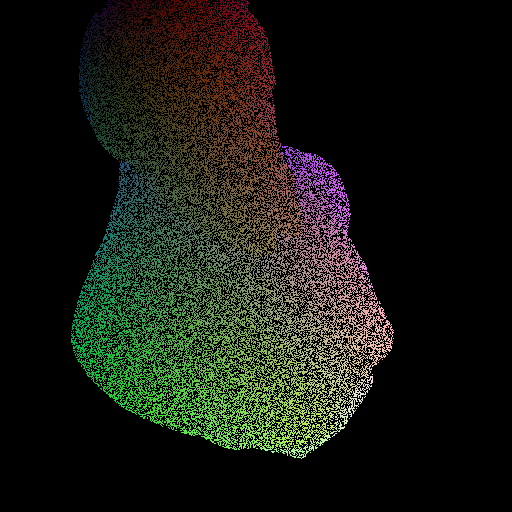
\includegraphics[width=.25\textwidth]{./Figures/train-input.png}};
		
		\draw [arrow] (oplus) -- (output);
		\draw [arrow] (sigmoid) |- (oplus);
		\draw [arrow] (LeakyReLU) -- (oplus);
		\draw [arrow] (conv2) --  node [text width=2.5cm, midway, right=1em]{LeakyReLU} (LeakyReLU);
		\draw [arrow] (conv1) --  node [text width=2.5cm, midway, right=1em]{Sigmoid} (sigmoid);
		\draw [arrow] (input) -|  node [text width=2.5cm, midway, below=1em]{Conv2D} (conv1);
		\draw [arrow] (input) -- node [text width=2.5cm, midway, right=1em]{Conv2D} (conv2);
	\end{tikzpicture}
	\caption{Gated Convolution Layer, where $ \oplus $ denotes element-wise multiplication.}
	\label{fig:gconvLayer}
\end{figure}

%\section{Canny Edge Detection for Detail Enhancement}
%The inaccuracy part is usually concentrate in the coarse surface or drastic changed surface parts of the object. The corresponding part can be extracted separately via edge detector algorithms, like Canny Edge detector. Feed the edges to a special net for normal prediction might improve the accuracy further. 

\subsection{Architecture}
\label{sec:architecture}
Based on the implementation mentioned above, the architecture roughly follows on UNet proposed by \cite{unet}, as shown in Figure \ref{fig:gcnn-archi}. 

Instead of using pooling layers for down/up samplings, gated convolution layer with stride $ (1,1) $ is used. The gated convolution using Sigmoid function for gating layer and LeakyReLU function for feature layer. All the layers are gated convolution layer with the exception of last two layers, which instead uses standard convolution layer to scale the output in range $\left[-1, 1\right]$. Other than the last two layers which use $ 1\times 1 $ kernels, all the gated convolution layer use $ 3\times 3 $ kernels with $ 1\times1 $ padding. 

The input is 3D vertex with size $ 512\times512\times3 $, and output is $ 512\times512\times3 $ normal map, which has the same resolution. There are 3 times downsamplings, each scale with 3 gated convolution layers, the third layer has stride 2. The upsampling part interpolate the feature maps 3 times with 1 gated convolution layer in each scale. 

It keeps the skip connection in UNet to remain the fine detail features. 
 
% GCNN Architecture
\begin{figure}[!h]
	\centering
	%% https://tex.stackexchange.com/questions/12020/what-is-the-easiest-way-to-draw-a-3d-cube-with-tikz
	\begin{tikzpicture}
		%% -------------------------------------- parameters ------------------------------------------------
		\pgfmathsetmacro{\vdist}{0.4}
		
		\pgfmathsetmacro{\boxsizea}{3}	%% width 512
		\pgfmathsetmacro{\boxsizeb}{1.5}	%% width 256
		\pgfmathsetmacro{\boxsizec}{1}	%% width 128
		\pgfmathsetmacro{\boxsized}{0.7}	%% width 64
		
		
		\pgfmathsetmacro{\boxwidthd}{0.1}	%% width 1
		\pgfmathsetmacro{\boxwidtha}{0.2}	%% width 3
		\pgfmathsetmacro{\boxwidthb}{\boxwidtha*1.3}	%% width 32
		\pgfmathsetmacro{\boxwidthc}{\boxwidtha*3}		%% width 64
		
		\pgfmathsetmacro{\convwshift}{9}
		\pgfmathsetmacro{\preprocessingshift}{4}
		\pgfmathsetmacro{\labelshift}{1.5}
		\pgfmathsetmacro{\gconvwshift}{0}
		
		\pgfmathsetmacro{\secrowshift}{-6}
		
		\pgfmathsetmacro{\convrowstart}{4}
		\pgfmathsetmacro{\secondrowstart}{4}
		
		%% https://www.tug.org/pracjourn/2007-4/walden/color.pdf
		\definecolor{gconvcolor}{rgb}{0.5,0.7,0.7}
		\definecolor{convcolor}{rgb}{0.5,0.7,0.3}
		\definecolor{gconvdilatedcolor}{rgb}{0.6,0,0.3}
		
		
		%% ---------------------------------- preprocessing --------------------------------------------
		%%  img_in 1x512x512
		\pgfmathsetmacro{\disttimes}{3.5}
		\pgfmathsetmacro{\yschift}{\preprocessingshift}
		\node[inner sep=0pt] (depthmap) at (\vdist*\disttimes,\yschift)
		{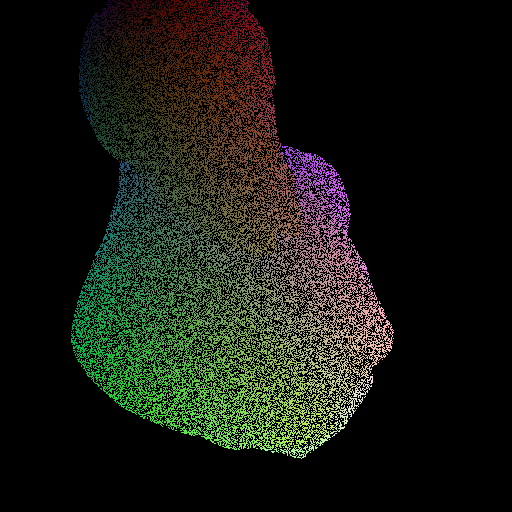
\includegraphics[width=.15\textwidth]{./Figures/train-input.png}};
		\node[text width=3.5cm] at (\vdist*\disttimes+1,\yschift-1.5) {3D Vertex};
		
		\draw [-stealth](1.45,\yschift-1.8) -- (1.45,\yschift-2.6);
		
		\draw [-stealth]  (\vdist*\disttimes+1.6,\yschift) -- (\vdist*\disttimes+1.1,\yschift);
		
		\pgfmathsetmacro{\disttimes}{10}
		\pgfmathsetmacro{\yschift}{\preprocessingshift}
		\node[inner sep=0pt] (depthmap) at (\vdist*\disttimes,\yschift)
		{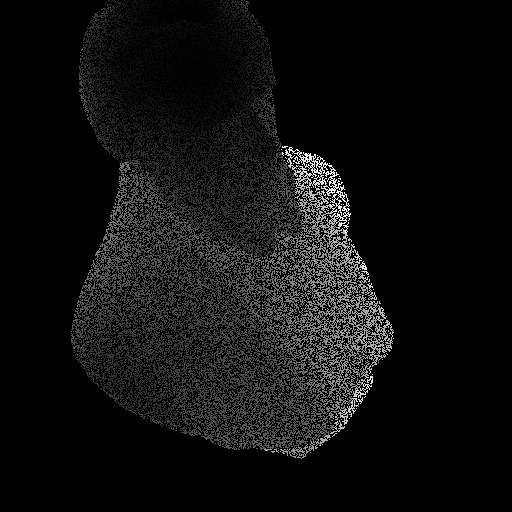
\includegraphics[width=.15\textwidth]{./Figures/train-depth-noise}};
		\node[text width=3.5cm] at (\vdist*\disttimes+1,\yschift-1.5) {Add Noise};
		
		\draw [-stealth] (\vdist*\disttimes+1.6,\yschift) -- (\vdist*\disttimes+1.1,\yschift);
		
		\pgfmathsetmacro{\disttimes}{16.5}
		\pgfmathsetmacro{\yschift}{\preprocessingshift}
		\node[inner sep=0pt] (depthmap) at (\vdist*\disttimes,\yschift)
		{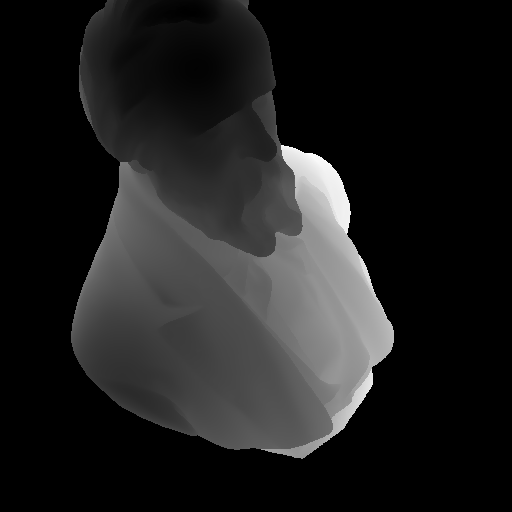
\includegraphics[width=.15\textwidth]{./Figures/train-depth.png}};
		\node[text width=2cm] at (\vdist*\disttimes+0.2,\yschift-1.5) {Depth Map};
		
		
		%% ----------------------------------- output normal map -------------------------------------
		\pgfmathsetmacro{\disttimes}{25}
		\pgfmathsetmacro{\yschift}{\preprocessingshift}
		\node[inner sep=0pt] (depthmap) at (\vdist*\disttimes,\yschift)
		{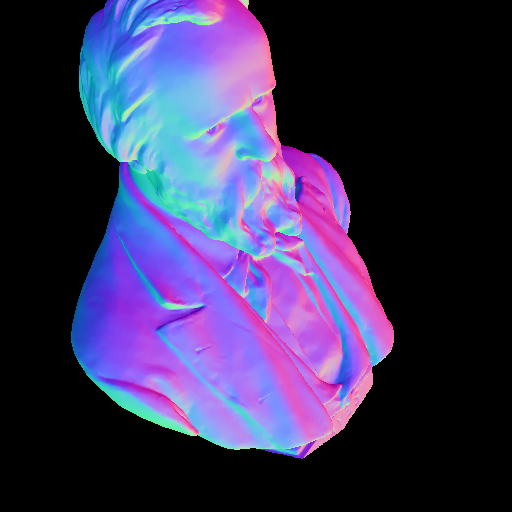
\includegraphics[width=.15\textwidth]{./Figures/train-normal-gt.png}};
		\node[text width=2.5cm] at (\vdist*\disttimes,\yschift-1.5) {Normal Map};
		
		\draw [-stealth] (\vdist*\disttimes+0.2,\yschift-2.7) -- (\vdist*\disttimes+0.2,\yschift-1.8);
		
		
		%% ------------------------------------------- vertex input ----------------------------------------------
		%% 	d_in							3x512x512
		%%	dconv1: 	d_in-->x1 			32x512x512
		\pgfmathsetmacro{\disttimes}{1}	%% width 32
		\pgfmathsetmacro{\boxsize}{\boxsizea}	%% size 512
		\pgfmathsetmacro{\boxwidth}{\boxwidthb}	%% width 32
		\pgfmathsetmacro{\yschift}{\gconvwshift}
		\draw[black, fill=gconvcolor] (\vdist*\disttimes,\yschift,0) -- ++(-\boxwidth,0,0) -- ++(0,-\boxsize,0) -- ++(\boxwidth,0,0) -- cycle;
		\draw[black, fill=gconvcolor] (\vdist*\disttimes,\yschift,0) -- ++(0,0,-\boxsize) -- ++(0,-\boxsize,0) -- ++(0,0,\boxsize) -- cycle;
		\draw[black, fill=gconvcolor] (\vdist*\disttimes,\yschift,0) -- ++(-\boxwidth,0,0) -- ++(0,0,-\boxsize) -- ++(\boxwidth,0,0) -- cycle;
		
		%%	dconv2:		x1-->x1				32x512x512
		\pgfmathsetmacro{\disttimes}{2}	%% width 32
		\pgfmathsetmacro{\boxsize}{\boxsizea}	%% size 512
		\pgfmathsetmacro{\boxwidth}{\boxwidthb}	%% width 32
		\pgfmathsetmacro{\yschift}{\gconvwshift}
		\draw[black, fill=gconvcolor] (\vdist*\disttimes,\yschift,0) -- ++(-\boxwidth,0,0) -- ++(0,-\boxsize,0) -- ++(\boxwidth,0,0) -- cycle;
		\draw[black, fill=gconvcolor] (\vdist*\disttimes,\yschift,0) -- ++(0,0,-\boxsize) -- ++(0,-\boxsize,0) -- ++(0,0,\boxsize) -- cycle;
		\draw[black, fill=gconvcolor] (\vdist*\disttimes,\yschift,0) -- ++(-\boxwidth,0,0) -- ++(0,0,-\boxsize) -- ++(\boxwidth,0,0) -- cycle;
		
		%%	dconv3:		x1-->x1				32x512x512
		\pgfmathsetmacro{\disttimes}{3}	%% width 32
		\pgfmathsetmacro{\boxsize}{\boxsizea}	%% size 512
		\pgfmathsetmacro{\boxwidth}{\boxwidthb}	%% width 32
		\pgfmathsetmacro{\yschift}{\gconvwshift}
		\draw[black, fill=gconvcolor] (\vdist*\disttimes,\yschift,0) -- ++(-\boxwidth,0,0) -- ++(0,-\boxsize,0) -- ++(\boxwidth,0,0) -- cycle;
		\draw[black, fill=gconvcolor] (\vdist*\disttimes,\yschift,0) -- ++(0,0,-\boxsize) -- ++(0,-\boxsize,0) -- ++(0,0,\boxsize) -- cycle;
		\draw[black, fill=gconvcolor] (\vdist*\disttimes,\yschift,0) -- ++(-\boxwidth,0,0) -- ++(0,0,-\boxsize) -- ++(\boxwidth,0,0) -- cycle;
		
		\draw (\vdist*\disttimes-0.2,\yschift-3.2) -- (\vdist*\disttimes-0.2,\yschift-4);
		\draw (\vdist*\disttimes-0.2,\yschift-4) -- (\vdist*\disttimes+6.5,\yschift-4);
		\draw [-stealth] (\vdist*\disttimes+6.5,\yschift-4) -- (\vdist*\disttimes+6.5,\yschift-3.2);
		
		
		%% downsample 1
		%%	dconv4:		x1-->x2				32x256x256
		\pgfmathsetmacro{\disttimes}{4}	%% width 32
		\pgfmathsetmacro{\boxsize}{\boxsizeb}	%% size 256
		\pgfmathsetmacro{\boxwidth}{\boxwidthb}	%% width 32
		\pgfmathsetmacro{\yschift}{\gconvwshift-0.5}	%% width 32
		\draw[black, fill=gconvcolor] (\vdist*\disttimes,\yschift,0) -- ++(-\boxwidth,0,0) -- ++(0,-\boxsize,0) -- ++(\boxwidth,0,0) -- cycle;
		\draw[black, fill=gconvcolor] (\vdist*\disttimes,\yschift,0) -- ++(0,0,-\boxsize) -- ++(0,-\boxsize,0) -- ++(0,0,\boxsize) -- cycle;
		\draw[black, fill=gconvcolor] (\vdist*\disttimes,\yschift,0) -- ++(-\boxwidth,0,0) -- ++(0,0,-\boxsize) -- ++(\boxwidth,0,0) -- cycle;
		%%	dconv2:		x2-->x2				32x256x256
		\pgfmathsetmacro{\disttimes}{5}	%% width 32
		\pgfmathsetmacro{\boxsize}{\boxsizeb}	%% size 256
		\pgfmathsetmacro{\boxwidth}{\boxwidthb}	%% width 32
		\pgfmathsetmacro{\yschift}{\gconvwshift-0.5}	%% width 32
		\draw[black, fill=gconvcolor] (\vdist*\disttimes,\yschift,0) -- ++(-\boxwidth,0,0) -- ++(0,-\boxsize,0) -- ++(\boxwidth,0,0) -- cycle;
		\draw[black, fill=gconvcolor] (\vdist*\disttimes,\yschift,0) -- ++(0,0,-\boxsize) -- ++(0,-\boxsize,0) -- ++(0,0,\boxsize) -- cycle;
		\draw[black, fill=gconvcolor] (\vdist*\disttimes,\yschift,0) -- ++(-\boxwidth,0,0) -- ++(0,0,-\boxsize) -- ++(\boxwidth,0,0) -- cycle;
		%%	dconv3:		x2-->x2				32x256x256
		\pgfmathsetmacro{\disttimes}{6}	%% width 32
		\pgfmathsetmacro{\boxsize}{\boxsizeb}	%% size 256
		\pgfmathsetmacro{\boxwidth}{\boxwidthb}	%% width 32
		\pgfmathsetmacro{\yschift}{\gconvwshift-0.5}	%% width 32
		\draw[black, fill=gconvcolor] (\vdist*\disttimes,\yschift,0) -- ++(-\boxwidth,0,0) -- ++(0,-\boxsize,0) -- ++(\boxwidth,0,0) -- cycle;
		\draw[black, fill=gconvcolor] (\vdist*\disttimes,\yschift,0) -- ++(0,0,-\boxsize) -- ++(0,-\boxsize,0) -- ++(0,0,\boxsize) -- cycle;
		\draw[black, fill=gconvcolor] (\vdist*\disttimes,\yschift,0) -- ++(-\boxwidth,0,0) -- ++(0,0,-\boxsize) -- ++(\boxwidth,0,0) -- cycle;
		
		\draw (\vdist*\disttimes-0.1,\yschift-1.6) -- (\vdist*\disttimes-0.1,\yschift-2.7);
		\draw (\vdist*\disttimes-0.1,\yschift-2.7) -- (\vdist*\disttimes+4.2,\yschift-2.7);
		\draw [-stealth] (\vdist*\disttimes+4.2,\yschift-2.7) -- (\vdist*\disttimes+4.2,\yschift-1.7);
		
		
		%% downsample 2
		%%	dconv4:		x2-->x3				32x128x128
		\pgfmathsetmacro{\disttimes}{7}	%% width 32
		\pgfmathsetmacro{\boxsize}{\boxsizec}	%% size 128
		\pgfmathsetmacro{\boxwidth}{\boxwidthb}	%% width 32
		\pgfmathsetmacro{\yschift}{\gconvwshift-0.8}	%% width 32
		\draw[black, fill=gconvcolor] (\vdist*\disttimes,\yschift,0) -- ++(-\boxwidth,0,0) -- ++(0,-\boxsize,0) -- ++(\boxwidth,0,0) -- cycle;
		\draw[black, fill=gconvcolor] (\vdist*\disttimes,\yschift,0) -- ++(0,0,-\boxsize) -- ++(0,-\boxsize,0) -- ++(0,0,\boxsize) -- cycle;
		\draw[black, fill=gconvcolor] (\vdist*\disttimes,\yschift,0) -- ++(-\boxwidth,0,0) -- ++(0,0,-\boxsize) -- ++(\boxwidth,0,0) -- cycle;
		%%	dconv2:		x3-->x3				32x128x128
		\pgfmathsetmacro{\disttimes}{8}	%% width 32
		\pgfmathsetmacro{\boxsize}{\boxsizec}	%% size 128
		\pgfmathsetmacro{\boxwidth}{\boxwidthb}	%% width 32
		\pgfmathsetmacro{\yschift}{\gconvwshift-0.8}	%% width 32
		\draw[black, fill=gconvcolor] (\vdist*\disttimes,\yschift,0) -- ++(-\boxwidth,0,0) -- ++(0,-\boxsize,0) -- ++(\boxwidth,0,0) -- cycle;
		\draw[black, fill=gconvcolor] (\vdist*\disttimes,\yschift,0) -- ++(0,0,-\boxsize) -- ++(0,-\boxsize,0) -- ++(0,0,\boxsize) -- cycle;
		\draw[black, fill=gconvcolor] (\vdist*\disttimes,\yschift,0) -- ++(-\boxwidth,0,0) -- ++(0,0,-\boxsize) -- ++(\boxwidth,0,0) -- cycle;
		%%	dconv3:		x3-->x3				32x128x128
		\pgfmathsetmacro{\disttimes}{9}	%% width 32
		\pgfmathsetmacro{\boxsize}{\boxsizec}	%% size 128
		\pgfmathsetmacro{\boxwidth}{\boxwidthb}	%% width 32
		\pgfmathsetmacro{\yschift}{\gconvwshift-0.8}	%% width 32
		\draw[black, fill=gconvcolor] (\vdist*\disttimes,\yschift,0) -- ++(-\boxwidth,0,0) -- ++(0,-\boxsize,0) -- ++(\boxwidth,0,0) -- cycle;
		\draw[black, fill=gconvcolor] (\vdist*\disttimes,\yschift,0) -- ++(0,0,-\boxsize) -- ++(0,-\boxsize,0) -- ++(0,0,\boxsize) -- cycle;
		\draw[black, fill=gconvcolor] (\vdist*\disttimes,\yschift,0) -- ++(-\boxwidth,0,0) -- ++(0,0,-\boxsize) -- ++(\boxwidth,0,0) -- cycle;
		
		\draw (\vdist*\disttimes-0.1,\yschift-1.2) -- (\vdist*\disttimes-0.1,\yschift-1.8);
		\draw (\vdist*\disttimes-0.1,\yschift-1.8) -- (\vdist*\disttimes+1.8,\yschift-1.8);
		\draw [-stealth] (\vdist*\disttimes+1.8,\yschift-1.8) -- (\vdist*\disttimes+1.8,\yschift-1.2);
		
		
		%% downsample 3
		%%	dconv4:		x3-->x4				32x64x64
		\pgfmathsetmacro{\disttimes}{10}
		\pgfmathsetmacro{\boxsize}{\boxsized}	%% size 64
		\pgfmathsetmacro{\boxwidth}{\boxwidthb}	%% width 32
		\pgfmathsetmacro{\yschift}{\gconvwshift-1}
		\draw[black, fill=gconvcolor] (\vdist*\disttimes,\yschift,0) -- ++(-\boxwidth,0,0) -- ++(0,-\boxsize,0) -- ++(\boxwidth,0,0) -- cycle;
		\draw[black, fill=gconvcolor] (\vdist*\disttimes,\yschift,0) -- ++(0,0,-\boxsize) -- ++(0,-\boxsize,0) -- ++(0,0,\boxsize) -- cycle;
		\draw[black, fill=gconvcolor] (\vdist*\disttimes,\yschift,0) -- ++(-\boxwidth,0,0) -- ++(0,0,-\boxsize) -- ++(\boxwidth,0,0) -- cycle;
		%%	dconv2:		x4-->x4				32x64x64
		\pgfmathsetmacro{\disttimes}{11}
		\pgfmathsetmacro{\boxsize}{\boxsized}	%% size 64
		\pgfmathsetmacro{\boxwidth}{\boxwidthb}	%% width 32
		\pgfmathsetmacro{\yschift}{\gconvwshift-1}	%% width 32
		\draw[black, fill=gconvcolor] (\vdist*\disttimes,\yschift,0) -- ++(-\boxwidth,0,0) -- ++(0,-\boxsize,0) -- ++(\boxwidth,0,0) -- cycle;
		\draw[black, fill=gconvcolor] (\vdist*\disttimes,\yschift,0) -- ++(0,0,-\boxsize) -- ++(0,-\boxsize,0) -- ++(0,0,\boxsize) -- cycle;
		\draw[black, fill=gconvcolor] (\vdist*\disttimes,\yschift,0) -- ++(-\boxwidth,0,0) -- ++(0,0,-\boxsize) -- ++(\boxwidth,0,0) -- cycle;
		%%	dconv3:		x4-->x4				32x64x64
		\pgfmathsetmacro{\disttimes}{12}
		\pgfmathsetmacro{\boxsize}{\boxsized}	%% size 64
		\pgfmathsetmacro{\boxwidth}{\boxwidthb}	%% width 32
		\pgfmathsetmacro{\yschift}{\gconvwshift-1}	%% width 32
		\draw[black, fill=gconvcolor] (\vdist*\disttimes,\yschift,0) -- ++(-\boxwidth,0,0) -- ++(0,-\boxsize,0) -- ++(\boxwidth,0,0) -- cycle;
		\draw[black, fill=gconvcolor] (\vdist*\disttimes,\yschift,0) -- ++(0,0,-\boxsize) -- ++(0,-\boxsize,0) -- ++(0,0,\boxsize) -- cycle;
		\draw[black, fill=gconvcolor] (\vdist*\disttimes,\yschift,0) -- ++(-\boxwidth,0,0) -- ++(0,0,-\boxsize) -- ++(\boxwidth,0,0) -- cycle;
		
		%		%% dilated
		%		%%	dilated1:	x4-->x4				32x64x64
		%		\pgfmathsetmacro{\disttimes}{13}
		%		\pgfmathsetmacro{\boxsize}{\boxsized}	%% size 64
		%		\pgfmathsetmacro{\boxwidth}{\boxwidthb}	%% width 32
		%		\pgfmathsetmacro{\yschift}{\gconvwshift-1}	%% width 32
		%		\draw[black, fill=gconvdilatedcolor] (\vdist*\disttimes,\yschift,0) -- ++(-\boxwidth,0,0) -- ++(0,-\boxsize,0) -- ++(\boxwidth,0,0) -- cycle;
		%		\draw[black, fill=gconvdilatedcolor] (\vdist*\disttimes,\yschift,0) -- ++(0,0,-\boxsize) -- ++(0,-\boxsize,0) -- ++(0,0,\boxsize) -- cycle;
		%		\draw[black, fill=gconvdilatedcolor] (\vdist*\disttimes,\yschift,0) -- ++(-\boxwidth,0,0) -- ++(0,0,-\boxsize) -- ++(\boxwidth,0,0) -- cycle;
		%		%%	dilated2:	x4-->x4				32x64x64
		%		\pgfmathsetmacro{\disttimes}{14}
		%		\pgfmathsetmacro{\boxsize}{\boxsized}	%% size 64
		%		\pgfmathsetmacro{\boxwidth}{\boxwidthb}	%% width 32
		%		\pgfmathsetmacro{\yschift}{\gconvwshift-1}	%% width 32
		%		\draw[black, fill=gconvdilatedcolor] (\vdist*\disttimes,\yschift,0) -- ++(-\boxwidth,0,0) -- ++(0,-\boxsize,0) -- ++(\boxwidth,0,0) -- cycle;
		%		\draw[black, fill=gconvdilatedcolor] (\vdist*\disttimes,\yschift,0) -- ++(0,0,-\boxsize) -- ++(0,-\boxsize,0) -- ++(0,0,\boxsize) -- cycle;
		%		\draw[black, fill=gconvdilatedcolor] (\vdist*\disttimes,\yschift,0) -- ++(-\boxwidth,0,0) -- ++(0,0,-\boxsize) -- ++(\boxwidth,0,0) -- cycle;
		%		%%	dilated3:	x4-->x4				32x64x64
		%		\pgfmathsetmacro{\disttimes}{15}
		%		\pgfmathsetmacro{\boxsize}{\boxsized}	%% size 64
		%		\pgfmathsetmacro{\boxwidth}{\boxwidthb}	%% width 32
		%		\pgfmathsetmacro{\yschift}{\gconvwshift-1}	%% width 32
		%		\draw[black, fill=gconvdilatedcolor] (\vdist*\disttimes,\yschift,0) -- ++(-\boxwidth,0,0) -- ++(0,-\boxsize,0) -- ++(\boxwidth,0,0) -- cycle;
		%		\draw[black, fill=gconvdilatedcolor] (\vdist*\disttimes,\yschift,0) -- ++(0,0,-\boxsize) -- ++(0,-\boxsize,0) -- ++(0,0,\boxsize) -- cycle;
		%		\draw[black, fill=gconvdilatedcolor] (\vdist*\disttimes,\yschift,0) -- ++(-\boxwidth,0,0) -- ++(0,0,-\boxsize) -- ++(\boxwidth,0,0) -- cycle;
		%		%%	dilated4:	x4-->x4				32x64x64
		%		\pgfmathsetmacro{\disttimes}{16}
		%		\pgfmathsetmacro{\boxsize}{\boxsized}	%% size 64
		%		\pgfmathsetmacro{\boxwidth}{\boxwidthb}	%% width 32
		%		\pgfmathsetmacro{\yschift}{\gconvwshift-1}	%% width 32
		%		\draw[black, fill=gconvdilatedcolor] (\vdist*\disttimes,\yschift,0) -- ++(-\boxwidth,0,0) -- ++(0,-\boxsize,0) -- ++(\boxwidth,0,0) -- cycle;
		%		\draw[black, fill=gconvdilatedcolor] (\vdist*\disttimes,\yschift,0) -- ++(0,0,-\boxsize) -- ++(0,-\boxsize,0) -- ++(0,0,\boxsize) -- cycle;
		%		\draw[black, fill=gconvdilatedcolor] (\vdist*\disttimes,\yschift,0) -- ++(-\boxwidth,0,0) -- ++(0,0,-\boxsize) -- ++(\boxwidth,0,0) -- cycle;
		%		
		%		
		%		
		%		
		%		%%	dconv2:		x4-->x4				32x64x64
		%		\pgfmathsetmacro{\disttimes}{17}
		%		\pgfmathsetmacro{\boxsize}{\boxsized}	%% size 64
		%		\pgfmathsetmacro{\boxwidth}{\boxwidthb}	%% width 32
		%		\pgfmathsetmacro{\yschift}{\gconvwshift-1}	%% width 32
		%		\draw[black, fill=gconvcolor] (\vdist*\disttimes,\yschift,0) -- ++(-\boxwidth,0,0) -- ++(0,-\boxsize,0) -- ++(\boxwidth,0,0) -- cycle;
		%		\draw[black, fill=gconvcolor] (\vdist*\disttimes,\yschift,0) -- ++(0,0,-\boxsize) -- ++(0,-\boxsize,0) -- ++(0,0,\boxsize) -- cycle;
		%		\draw[black, fill=gconvcolor] (\vdist*\disttimes,\yschift,0) -- ++(-\boxwidth,0,0) -- ++(0,0,-\boxsize) -- ++(\boxwidth,0,0) -- cycle;
		%		%%	dconv3:		x4-->x4				32x64x64
		%		\pgfmathsetmacro{\disttimes}{18}
		%		\pgfmathsetmacro{\boxsize}{\boxsized}	%% size 64
		%		\pgfmathsetmacro{\boxwidth}{\boxwidthb}	%% width 32
		%		\pgfmathsetmacro{\yschift}{\gconvwshift-1}	%% width 32
		%		\draw[black, fill=gconvcolor] (\vdist*\disttimes,\yschift,0) -- ++(-\boxwidth,0,0) -- ++(0,-\boxsize,0) -- ++(\boxwidth,0,0) -- cycle;
		%		\draw[black, fill=gconvcolor] (\vdist*\disttimes,\yschift,0) -- ++(0,0,-\boxsize) -- ++(0,-\boxsize,0) -- ++(0,0,\boxsize) -- cycle;
		%		\draw[black, fill=gconvcolor] (\vdist*\disttimes,\yschift,0) -- ++(-\boxwidth,0,0) -- ++(0,0,-\boxsize) -- ++(\boxwidth,0,0) -- cycle;
		
		
		%% ----------------------------------- upsampling -------------------------------------
		
		%% upsample 1
		%% interpolate	x4-->x3_us			64x128x128
		\pgfmathsetmacro{\disttimes}{13}
		\pgfmathsetmacro{\boxsize}{\boxsizec}	%% size 128
		\pgfmathsetmacro{\boxwidth}{\boxwidthb}	%% width 32
		\pgfmathsetmacro{\yschift}{\gconvwshift-0.9}	%% width 32
		\draw[black, fill=gconvcolor] (\vdist*\disttimes,\yschift,0) -- ++(-\boxwidth,0,0) -- ++(0,-\boxsize,0) -- ++(\boxwidth,0,0) -- cycle;
		\draw[black, fill=gconvcolor] (\vdist*\disttimes,\yschift,0) -- ++(0,0,-\boxsize) -- ++(0,-\boxsize,0) -- ++(0,0,\boxsize) -- cycle;
		\draw[black, fill=gconvcolor] (\vdist*\disttimes,\yschift,0) -- ++(-\boxwidth,0,0) -- ++(0,0,-\boxsize) -- ++(\boxwidth,0,0) -- cycle;
		
		%% concatenate x3_us
		\pgfmathsetmacro{\boxsize}{\boxsizec}	%% size 128
		\pgfmathsetmacro{\boxwidth}{\boxwidthb}	%% width 32
		\pgfmathsetmacro{\yschift}{\gconvwshift-0.9}	%% width 32
		\draw[black, fill=gconvcolor] (\vdist*\disttimes+\boxwidth,\yschift,0) -- ++(-\boxwidth,0,0) -- ++(0,-\boxsize,0) -- ++(\boxwidth,0,0) -- cycle;
		\draw[black, fill=gconvcolor] (\vdist*\disttimes+\boxwidth,\yschift,0) -- ++(0,0,-\boxsize) -- ++(0,-\boxsize,0) -- ++(0,0,\boxsize) -- cycle;
		\draw[black, fill=gconvcolor] (\vdist*\disttimes+\boxwidth,\yschift,0) -- ++(-\boxwidth,0,0) -- ++(0,0,-\boxsize) -- ++(\boxwidth,0,0) -- cycle;
		
		%% uconv1		x3_us-->x3			32x128x128
		\pgfmathsetmacro{\disttimes}{15}
		\pgfmathsetmacro{\boxsize}{\boxsizec}	%% size 128
		\pgfmathsetmacro{\boxwidth}{\boxwidthb}	%% width 32
		\pgfmathsetmacro{\yschift}{\gconvwshift-0.9}	%% width 32
		\draw[black, fill=gconvcolor] (\vdist*\disttimes,\yschift,0) -- ++(-\boxwidth,0,0) -- ++(0,-\boxsize,0) -- ++(\boxwidth,0,0) -- cycle;
		\draw[black, fill=gconvcolor] (\vdist*\disttimes,\yschift,0) -- ++(0,0,-\boxsize) -- ++(0,-\boxsize,0) -- ++(0,0,\boxsize) -- cycle;
		\draw[black, fill=gconvcolor] (\vdist*\disttimes,\yschift,0) -- ++(-\boxwidth,0,0) -- ++(0,0,-\boxsize) -- ++(\boxwidth,0,0) -- cycle;
		
		%% upsample 2
		%% interpolate	x3-->x2_us			32x256x256
		\pgfmathsetmacro{\disttimes}{16}
		\pgfmathsetmacro{\boxsize}{\boxsizeb}	%% size 256
		\pgfmathsetmacro{\boxwidth}{\boxwidthb}	%% width 32
		\pgfmathsetmacro{\yschift}{\gconvwshift-0.6}	%% width 32
		\draw[black, fill=gconvcolor] (\vdist*\disttimes,\yschift,0) -- ++(-\boxwidth,0,0) -- ++(0,-\boxsize,0) -- ++(\boxwidth,0,0) -- cycle;
		\draw[black, fill=gconvcolor] (\vdist*\disttimes,\yschift,0) -- ++(0,0,-\boxsize) -- ++(0,-\boxsize,0) -- ++(0,0,\boxsize) -- cycle;
		\draw[black, fill=gconvcolor] (\vdist*\disttimes,\yschift,0) -- ++(-\boxwidth,0,0) -- ++(0,0,-\boxsize) -- ++(\boxwidth,0,0) -- cycle;
		%% concatenated x2
		\pgfmathsetmacro{\boxsize}{\boxsizeb}	%% size 256
		\pgfmathsetmacro{\boxwidth}{\boxwidthb}	%% width 32
		\pgfmathsetmacro{\yschift}{\gconvwshift-0.6}	%% width 32
		\draw[black, fill=gconvcolor] (\vdist*\disttimes+\boxwidth,\yschift,0) -- ++(-\boxwidth,0,0) -- ++(0,-\boxsize,0) -- ++(\boxwidth,0,0) -- cycle;
		\draw[black, fill=gconvcolor] (\vdist*\disttimes+\boxwidth,\yschift,0) -- ++(0,0,-\boxsize) -- ++(0,-\boxsize,0) -- ++(0,0,\boxsize) -- cycle;
		\draw[black, fill=gconvcolor] (\vdist*\disttimes+\boxwidth,\yschift,0) -- ++(-\boxwidth,0,0) -- ++(0,0,-\boxsize) -- ++(\boxwidth,0,0) -- cycle;
		
		%% uconv2 		x2,x2_us-->x2		32x256x256
		\pgfmathsetmacro{\disttimes}{18}
		\pgfmathsetmacro{\boxsize}{\boxsizeb}	%% size 256
		\pgfmathsetmacro{\boxwidth}{\boxwidthb}	%% width 32
		\pgfmathsetmacro{\yschift}{\gconvwshift-0.6}	%% width 32
		\draw[black, fill=gconvcolor] (\vdist*\disttimes,\yschift,0) -- ++(-\boxwidth,0,0) -- ++(0,-\boxsize,0) -- ++(\boxwidth,0,0) -- cycle;
		\draw[black, fill=gconvcolor] (\vdist*\disttimes,\yschift,0) -- ++(0,0,-\boxsize) -- ++(0,-\boxsize,0) -- ++(0,0,\boxsize) -- cycle;
		\draw[black, fill=gconvcolor] (\vdist*\disttimes,\yschift,0) -- ++(-\boxwidth,0,0) -- ++(0,0,-\boxsize) -- ++(\boxwidth,0,0) -- cycle;
		
		
		%% upsample 3
		%% interpolate	x2-->x1_us			32x512x512
		\pgfmathsetmacro{\disttimes}{19}
		\pgfmathsetmacro{\boxsize}{\boxsizea}	%% size 512
		\pgfmathsetmacro{\boxwidth}{\boxwidthb}	%% width 32
		\pgfmathsetmacro{\yschift}{\gconvwshift}	%% width 32
		\draw[black, fill=gconvcolor] (\vdist*\disttimes,\yschift,0) -- ++(-\boxwidth,0,0) -- ++(0,-\boxsize,0) -- ++(\boxwidth,0,0) -- cycle;
		\draw[black, fill=gconvcolor] (\vdist*\disttimes,\yschift,0) -- ++(0,0,-\boxsize) -- ++(0,-\boxsize,0) -- ++(0,0,\boxsize) -- cycle;
		\draw[black, fill=gconvcolor] (\vdist*\disttimes,\yschift,0) -- ++(-\boxwidth,0,0) -- ++(0,0,-\boxsize) -- ++(\boxwidth,0,0) -- cycle;
		%% concatenated x1 and x1_us
		\pgfmathsetmacro{\boxsize}{\boxsizea}	%% size 512
		\pgfmathsetmacro{\boxwidth}{\boxwidthb}	%% width 32
		\pgfmathsetmacro{\yschift}{\gconvwshift}	%% width 32
		\draw[black, fill=gconvcolor] (\vdist*\disttimes+\boxwidth,\yschift,0) -- ++(-\boxwidth,0,0) -- ++(0,-\boxsize,0) -- ++(\boxwidth,0,0) -- cycle;
		\draw[black, fill=gconvcolor] (\vdist*\disttimes+\boxwidth,\yschift,0) -- ++(0,0,-\boxsize) -- ++(0,-\boxsize,0) -- ++(0,0,\boxsize) -- cycle;
		\draw[black, fill=gconvcolor] (\vdist*\disttimes+\boxwidth,\yschift,0) -- ++(-\boxwidth,0,0) -- ++(0,0,-\boxsize) -- ++(\boxwidth,0,0) -- cycle;
		
		
		%% uconv3		x1,x1_us-->x1		32x512x512
		\pgfmathsetmacro{\disttimes}{21}
		\pgfmathsetmacro{\boxsize}{\boxsizea}	%% size 512
		\pgfmathsetmacro{\boxwidth}{\boxwidthb}	%% width 32
		\pgfmathsetmacro{\yschift}{\gconvwshift}	%% width 32
		\draw[black, fill=gconvcolor] (\vdist*\disttimes,\yschift,0) -- ++(-\boxwidth,0,0) -- ++(0,-\boxsize,0) -- ++(\boxwidth,0,0) -- cycle;
		\draw[black, fill=gconvcolor] (\vdist*\disttimes,\yschift,0) -- ++(0,0,-\boxsize) -- ++(0,-\boxsize,0) -- ++(0,0,\boxsize) -- cycle;
		\draw[black, fill=gconvcolor] (\vdist*\disttimes,\yschift,0) -- ++(-\boxwidth,0,0) -- ++(0,0,-\boxsize) -- ++(\boxwidth,0,0) -- cycle;
		
		%% conv1		x1-->xout			3x512x512
		\pgfmathsetmacro{\disttimes}{22}
		\pgfmathsetmacro{\boxsize}{\boxsizea}	%% size 512
		\pgfmathsetmacro{\boxwidth}{\boxwidthb}	%% width 3
		\pgfmathsetmacro{\yschift}{\gconvwshift}	%% width 32
		\draw[black, fill=convcolor] (\vdist*\disttimes,\yschift,0) -- ++(-\boxwidth,0,0) -- ++(0,-\boxsize,0) -- ++(\boxwidth,0,0) -- cycle;
		\draw[black, fill=convcolor] (\vdist*\disttimes,\yschift,0) -- ++(0,0,-\boxsize) -- ++(0,-\boxsize,0) -- ++(0,0,\boxsize) -- cycle;
		\draw[black, fill=convcolor] (\vdist*\disttimes,\yschift,0) -- ++(-\boxwidth,0,0) -- ++(0,0,-\boxsize) -- ++(\boxwidth,0,0) -- cycle;
		
		
		
		%% conv2		xout-->xout			3x512x512
		\pgfmathsetmacro{\disttimes}{23}
		\pgfmathsetmacro{\boxsize}{\boxsizea}	%% size 512
		\pgfmathsetmacro{\boxwidth}{\boxwidthd}	%% width 3
		\pgfmathsetmacro{\yschift}{\gconvwshift}	%% width 32
		\node[text width=1cm] at (\vdist*\disttimes+0.5,\yschift-3.3) {3};
		\draw[black, fill=convcolor] (\vdist*\disttimes,\yschift,0) -- ++(-\boxwidth,0,0) -- ++(0,-\boxsize,0) -- ++(\boxwidth,0,0) -- cycle;
		\draw[black, fill=convcolor] (\vdist*\disttimes,\yschift,0) -- ++(0,0,-\boxsize) -- ++(0,-\boxsize,0) -- ++(0,0,\boxsize) -- cycle;
		\draw[black, fill=convcolor] (\vdist*\disttimes,\yschift,0) -- ++(-\boxwidth,0,0) -- ++(0,0,-\boxsize) -- ++(\boxwidth,0,0) -- cycle;
		
		
		%% ------------------------------------- label ----------------------------------------------		
		\pgfmathsetmacro{\disttimes}{10}
		\pgfmathsetmacro{\boxsize}{\boxsized}	%% size 512
		\pgfmathsetmacro{\boxwidth}{\boxwidthc}	%% width 3
		\pgfmathsetmacro{\yschift}{\labelshift}	%% width 32
		\node[text width=3.5cm] at (\vdist*\disttimes+1,\yschift-1) {Conv2d};
		\draw[black, fill=convcolor] (\vdist*\disttimes,\yschift,0) -- ++(-\boxwidth,0,0) -- ++(0,-\boxsize,0) -- ++(\boxwidth,0,0) -- cycle;
		\draw[black, fill=convcolor] (\vdist*\disttimes,\yschift,0) -- ++(0,0,-\boxsize) -- ++(0,-\boxsize,0) -- ++(0,0,\boxsize) -- cycle;
		\draw[black, fill=convcolor] (\vdist*\disttimes,\yschift,0) -- ++(-\boxwidth,0,0) -- ++(0,0,-\boxsize) -- ++(\boxwidth,0,0) -- cycle;
		
		\pgfmathsetmacro{\disttimes}{15}
		\pgfmathsetmacro{\boxsize}{\boxsized}	%% size 512
		\pgfmathsetmacro{\boxwidth}{\boxwidthc}	%% width 3
		\pgfmathsetmacro{\yschift}{\labelshift}	%% width 32
		\node[text width=3.5cm] at (\vdist*\disttimes+1,\yschift-1) {Gated};
		\draw[black, fill=gconvcolor] (\vdist*\disttimes,\yschift,0) -- ++(-\boxwidth,0,0) -- ++(0,-\boxsize,0) -- ++(\boxwidth,0,0) -- cycle;
		\draw[black, fill=gconvcolor] (\vdist*\disttimes,\yschift,0) -- ++(0,0,-\boxsize) -- ++(0,-\boxsize,0) -- ++(0,0,\boxsize) -- cycle;
		\draw[black, fill=gconvcolor] (\vdist*\disttimes,\yschift,0) -- ++(-\boxwidth,0,0) -- ++(0,0,-\boxsize) -- ++(\boxwidth,0,0) -- cycle;
		
		
		
	\end{tikzpicture}
	
	\caption{Basic Normal Neural Network model based on Gated Convolution layer and UNet architecture. }
	\label{fig:gcnn-archi}
\end{figure}

\subsection{Loss Function}

\paragraph{L1 Loss}
L1 loss, also known as absolute error loss, which calculates the absolute difference between the prediction and the ground truth. It leads to the median of the observations.

\[ L_1(\tilde y - y) = |\tilde y - y | \]

\paragraph{L2 Loss}
The standard loss function for optimization in regression problems is the L2 loss, also known as squared error loss, which minimize the squared difference between a prediction and the actual value. It leads to the mean of the observations. 
\[ L_2(\tilde y - y) = \|\tilde y - y \|_2^2 \]


\paragraph{Masked L2 Loss with penalty for outliers(mask-l2)}
\label{par:maskl2}
The background pixels of the input data are not considered in the normal inference task, they are saved as black pixels in the input data. These pixels should not considered in the loss function, i.e. invalid pixels. Therefore, a valid mask is required to distinguish the background and the main object. Specifically, using a matrix with the same width and height as the output, for each pixel, 0 is invalid, 1 is valid. 
Furthermore, depends on the specific task, the output should be constraint in a range. For normal output, the range is $ [-1,1] $. Thus for the outliers out of this range, a outlier mask can be applied to give them a penalty.

\begin{equation}\label{gcnn-loss}
	\begin{array}{ll}
		l(x,y)&= L  = \{l_1, ..., l_N\}^T\\ 
		l_{n\in N} &= \| mask_{obj} \odot mask_{ol} \odot ( {\tilde y}_n - y_n) \|_2^2 + 	\| mask_{obj} \odot mask_{nol} \odot ( {\tilde y}_n - y_n) \|_2^2 \\
	\end{array}
\end{equation}

where $ x $ is input, $ y $ is target, $ N $ is the batch size.$ mask_{obj} $ is the mask of the object, i.e. 1 means it is an pixel on the object, 0 is an pixel on the background. $ mask_{ol} $ is the mask for the outliers, i.e. 1 means outliers, 0 means non outlier, $ mask_{nol} $ is exactly the inverse of $ mask_{ol} $. $ p $ is the penalty of the outliers, it is set as 1.4.


\paragraph{Reversed Huber Loss}

\cite{berhu-loss} proposed Reversed Huber loss to combine both L1 and L2 loss. L1 loss is for small values whereas L2 for large values
\begin{equation}\label{berhu-loss}
	\begin{array}{ll}
		\mathcal{B}(y)= \begin{cases}
			|y| & |y| \le c \\
			\dfrac{y^2 + c^2}{2d} & |x| > c\\
		\end{cases}
	\end{array}
\end{equation}
where $ c=0.2\max (|\tilde y - y|) $.




\newpage
	
\section{Guided normal inference using GCNN}

\subsection{Intrinsic image decomposition}
Intrinsic image model was introduced by \cite{intrinsic-image}. It interprets that an image $ I $ can be decomposed as the element-wise product between the reflectance $ R $ of the object and the shading $ S $ produced by the interaction between light and objects.
\[ I =R  \odot S\]
It interprets the observed image into reflectance image and the shading image. As shown in Figure \ref{fig:intrinsic-image}
%% insert a image for decompositions
\begin{figure}[th]
	\centering
	{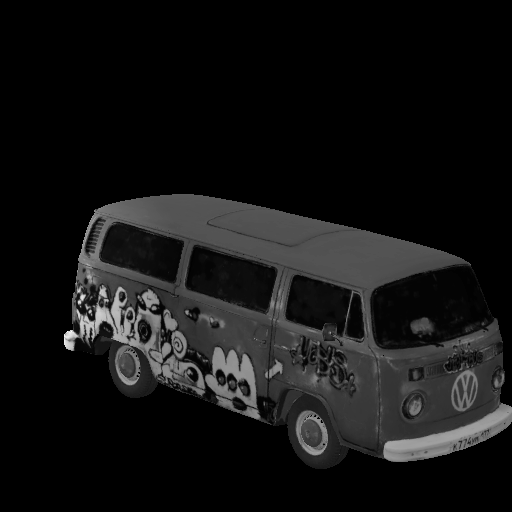
\includegraphics[width=.18\textwidth]{./Figures/intrinsic_image.png}}
	{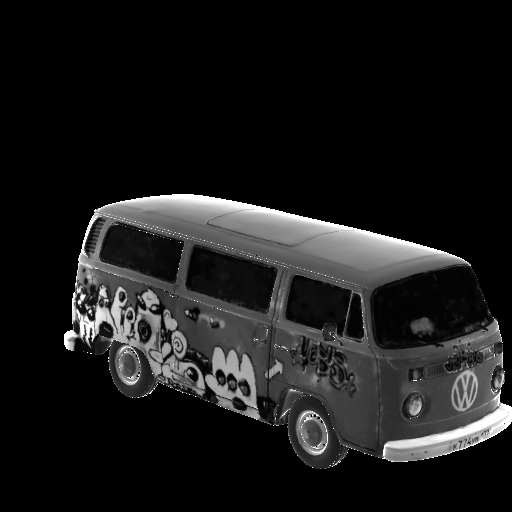
\includegraphics[width=.18\textwidth]{./Figures/intrinsic_image_reflectance.png}}
	{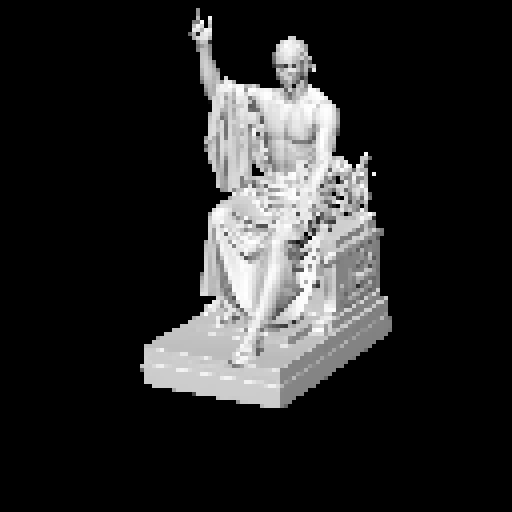
\includegraphics[width=.18\textwidth]{./Figures/intrinsic_image_shading.png}}
	{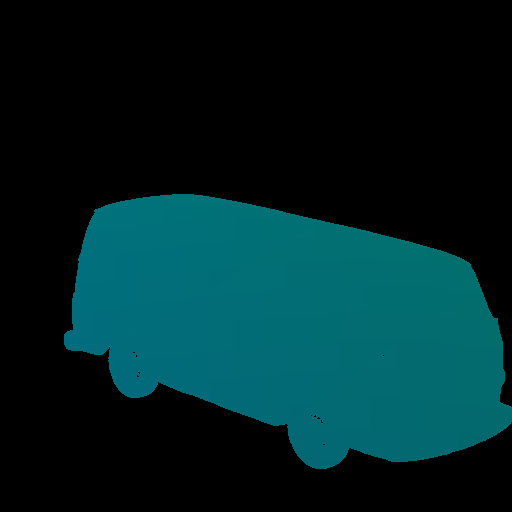
\includegraphics[width=.18\textwidth]{./Figures/intrinsic_image_light.png}}
	{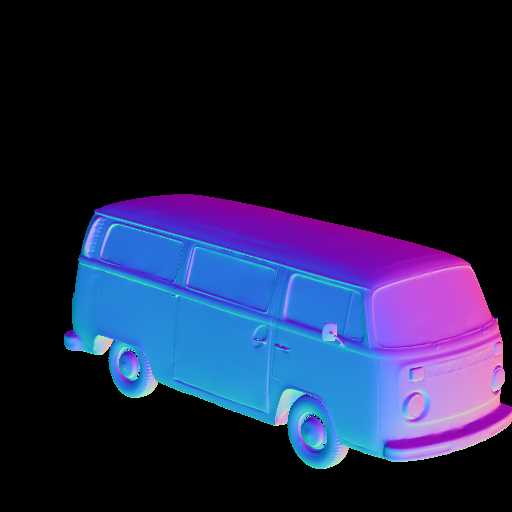
\includegraphics[width=.18\textwidth]{./Figures/intrinsic_image_normal.png}}
	\caption{Intrinsic image analysis of the bus object. From left to right, original image, reflectance image, shading image, light image, normal image}
	\label{fig:intrinsic-image}
\end{figure}

The equation can be further decomposed based on different surface models. If assume the object surfaces are Lambertian surfaces, i.e. the surface which reflect light in all directions, the shading image can be decomposed as the product of the  radiance of  incoming light $ L_0 $, the cosine of the angle of incidence, which is the dot product of the surface normal $ N $ and the light source direction $ L $.
\[ I = \rho  \odot ( L_0 \textbf{L} \cdot  \textbf{N}) \]
note that the surface normal $ N $ and light direction $ L $ are unit vectors thus they have only two degrees of freedom. 

\begin{figure}[th]
	\centering
	\begin{tikzpicture} 
		% reference lines
		\coordinate (light) at (-1,3);
		\coordinate (p) at (2,0);
		\coordinate (normal) at (2,3);
		\draw [fill=blue!20] plot [smooth cycle] coordinates {(0,0) (1,1) (3,1) (5,0) (2,-1)}; %% surface element
		\draw[thick, ->] (2,0) -- (2,3) node[midway, left] {$ \textbf{n} $}; %% normal
		\draw[thick, ->] (2,0) -- (-1,3) node[midway, left] {$ \textbf{l} $}  ; %% source direction
		\pic [draw, ->, "$\theta$", angle eccentricity=1.5] {angle = normal--p--light};
		\draw[thick, ->] (2,0) -- (5,3) node[midway, left] {$ \textbf{v} $}; %% view direction
		\filldraw[black] (-1,3) circle (2pt) node[anchor=south west]{light source}; %% light source
		\filldraw[black] (5,3) circle (2pt) node[anchor=south west]{view point}; %% view point		
	\end{tikzpicture}
	\caption{The surface normal, source light direction and the view point direction, where $ \theta $ denotes the angle between light direction and the normal.}
	\label{fig:lambertian-surface}
\end{figure}

The equation can be further rearranged as follows
\[ I = \textbf{g} \cdot \textbf{L} =(L_0\rho \odot \textbf{N}) \cdot  ( \textbf{L}) \]
The shape from shading method employed the equation mentioned above to predict the both surface albedo $ \rho $ and the normal $ \textbf{N} $ with knowning light source direction $ \textbf{L} $. More specifically, a set of $ k $ image for the same scene have been captured based on different light projections. Then, for each pixel $ (x,y) $ in the image, an equation system can be set up 

\[ 
\begin{pmatrix}
	L_1^T \\
	L_2^T \\
	\cdots \\
	L_k^T
\end{pmatrix} g(x,y) = 
\begin{pmatrix}
	I_1(x,y) \\
	I_2(x,y) \\
	\cdots \\
	I_3(x,y)
\end{pmatrix}
\]
for the simplicity, $ L_i^T $ for $ 1\le i \le k $ denotes the light direction at position $ (x,y) $ in the image $ k $ 
The equation can be solved based on least square methods. 
Since normal $ N(x,y) $ is unit vector, thus we have 

\[ \|g(x,y)\|_2 = \|L_0\rho(x,y)N(x,y)\|_2 = L_0\rho(x,y) \]

Then the normal can be obtained as follow

\[  N(x,y) = \frac{g(x,y)}{L_0\rho(x,y)}\]

In another word, the surface normal including the albedo can be obtained directly based on images and light directions. 


\subsection{Light Map}
\label{sec:lightmap}
The light map $ L $ can be derived from vertex map and the light source position. As shown in Figure \ref{fig:lambertian-surface}, the incoming light direction is a vector point from light source to the surface point, therefor it can be calculated as follows
\begin{equation}\label{light-direction}
	\begin{array}{ll}
		L(x,y)&= \dfrac{V(x,y)-(s_x,s_y)}{\|V(x,y)-(s_x,s_y)\|_2}\\ 
	\end{array}
\end{equation}
where $ (s_x,s_y) $ is the light source position and $ V $ is the vertices, both $  (s_x,s_y) $ and  $ V $ are with respect to the camera space. The light direction map $ L $ is normalized since only the direction of the light is considered. 
The light map is a matrix corresponding the light direction of whole image where each pixel corresponding with each other, thus it has the same size as the vertex map.


It is important to note that due to the exist noise in the vertex map, the getting light map is only semi-dense, as shown in Figure \ref{fig:light-input}. 

\begin{figure}[th]
	\centering
	{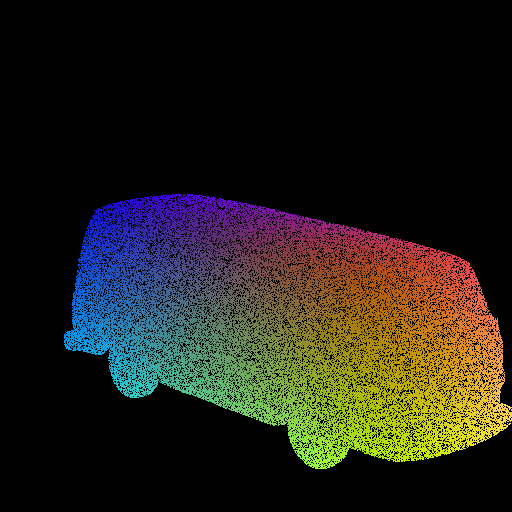
\includegraphics[width=.4\textwidth]{./Figures/intrinsic_image_vertex_input.png}}
	{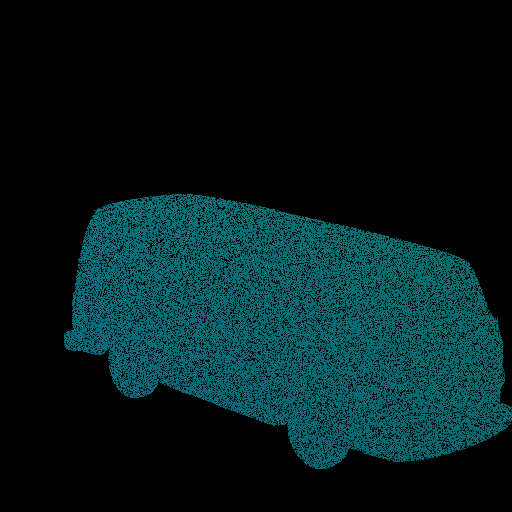
\includegraphics[width=.4\textwidth]{./Figures/intrinsic_image_light_input.png}}
	\caption{The light map calculated from vertex map and the light source}
	\label{fig:light-input}
\end{figure}

In order to ease this issue, a light inpainting model has been trained based on the GCNN network with the identity architecture but the input and output, which takes the semi-dense light map as input and predict the fully dense light map as output. 

\begin{figure}[th]
	\centering
	%% https://tex.stackexchange.com/questions/12020/what-is-the-easiest-way-to-draw-a-3d-cube-with-tikz
	\begin{tikzpicture}
		%% -------------------------------------- parameters ------------------------------------------------
		\pgfmathsetmacro{\vdist}{0.4}
		
		\pgfmathsetmacro{\boxsizea}{2}	%% width 512
		\pgfmathsetmacro{\boxwidtha}{2}	%% width 3
		
		%% https://www.tug.org/pracjourn/2007-4/walden/color.pdf
		\definecolor{netcolor}{rgb}{0.5,0.7,0.7}
		
		%% 	d_in							3x512x512
		%%	dconv1: 	d_in-->x1 			32x512x512
		\pgfmathsetmacro{\disttimes}{1}	%% width 32
		\pgfmathsetmacro{\yshift}{1}	%% width 32
		\pgfmathsetmacro{\boxsize}{\boxsizea}	%% size 512
		\pgfmathsetmacro{\boxwidth}{\boxwidtha}	%% width 32
		\pgfmathsetmacro{\yschift}{-1}
		
		
		\node[inner sep=0pt] (input) at (\vdist*\disttimes-6,\yschift-0.8)
		{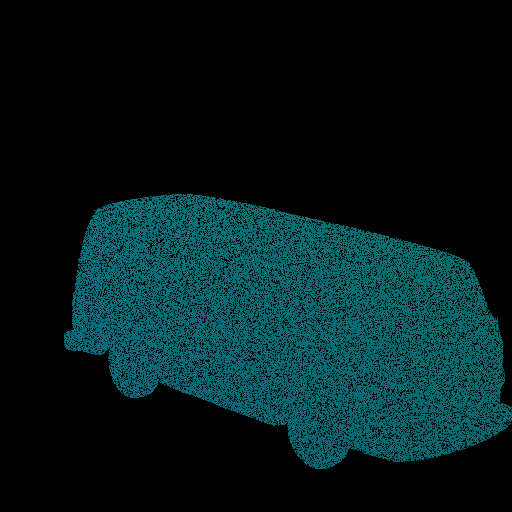
\includegraphics[width=.2\textwidth]{./Figures/intrinsic_image_light_input.png}};
		\node[text width=3.5cm] at (\vdist*\disttimes-6,\yschift-2.4) {Semi-dense Light Map};
		
		\node[inner sep=0pt] (output) at (\vdist*\disttimes+3,\yschift-0.8)
		{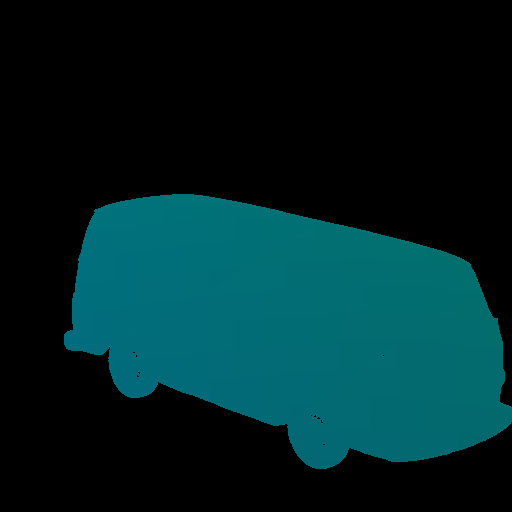
\includegraphics[width=.2\textwidth]{./Figures/intrinsic_image_light.png}};
		\node[text width=3.5cm] at (\vdist*\disttimes+3,\yschift-2.4) {Semi-dense Light Map};
		
		\draw [-stealth] (\vdist*\disttimes-4.5,\yschift-1) -- (\vdist*\disttimes-3.5,\yschift-1);
		\draw [-stealth] (\vdist*\disttimes,\yschift-1) -- (\vdist*\disttimes+1,\yschift-1);
		
		
		\pgfmathsetmacro{\disttimes}{-2}	%% width 32		
		\pgfmathsetmacro{\yschift}{-1}
		\draw[black, fill=netcolor] (\vdist*\disttimes,\yschift,0) -- ++(-\boxwidth,0,0) -- ++(0,-\boxsize,0) -- ++(\boxwidth,0,0) -- cycle;
		\draw[black, fill=netcolor] (\vdist*\disttimes,\yschift,0) -- ++(0,0,-\boxsize) -- ++(0,-\boxsize,0) -- ++(0,0,\boxsize) -- cycle;
		\draw[black, fill=netcolor] (\vdist*\disttimes,\yschift,0) -- ++(-\boxwidth,0,0) -- ++(0,0,-\boxsize) -- ++(\boxwidth,0,0) -- cycle;
		
		\node[text width=3.5cm] at (\vdist*\disttimes,\yschift-1) {Light Net};
	\end{tikzpicture}
	\caption{Light Net for light inpainting based on GCNN architecture.}
	\label{fig:light-net-archi}
\end{figure}


\subsection{Light and image guided normal inference using GCNN}
Based on above implementations, we propose a light and image guided network called Vertex-Image-Light Network (VIL-Net). 
The structure is shown in Figure \ref{fig:albedo-gated-archi}. As mentioned in the name, the network utilizes the GCNN architecture three times to accomplish the task. The first branch (shown above) takes a light map introduced in \ref{sec:lightmap} as the input, the structure is the same as GCNN architecture except that the last two standard convolution layers, the skip connections are kept to connect the 3 down/up samplings. 
The second branch (shown below) takes image as the input, the structure is the same as the first branch other than the input image is 1 channel but not 3 channels. 
The third branch takes the 3D vertex map as the input. The structure is based on GCNN architecture. However, in order to merge the other two branches, the vertex branch equips 4 times fusions in the up sampling part. Specifically, the first fusion locates immediately after the last gconv layer of the last down sampling, the second fusion after the second gconv layer of first up sampling, the third fusion after the second gconv layer of second up sampling, the fourth fusion after the second gconv layer of the third up sampling. Each fusion follows by an interpolation layer, a gconv layer to reduce the channel back to 32, a skip connection concatenate layer and another gconv layer to reduce the channel back to 32. After the fourth fusion, a gconv layer used for channel reduction, 2 standard conv layer for output prediction.

\begin{sidewaysfigure}[th]
	\centering
	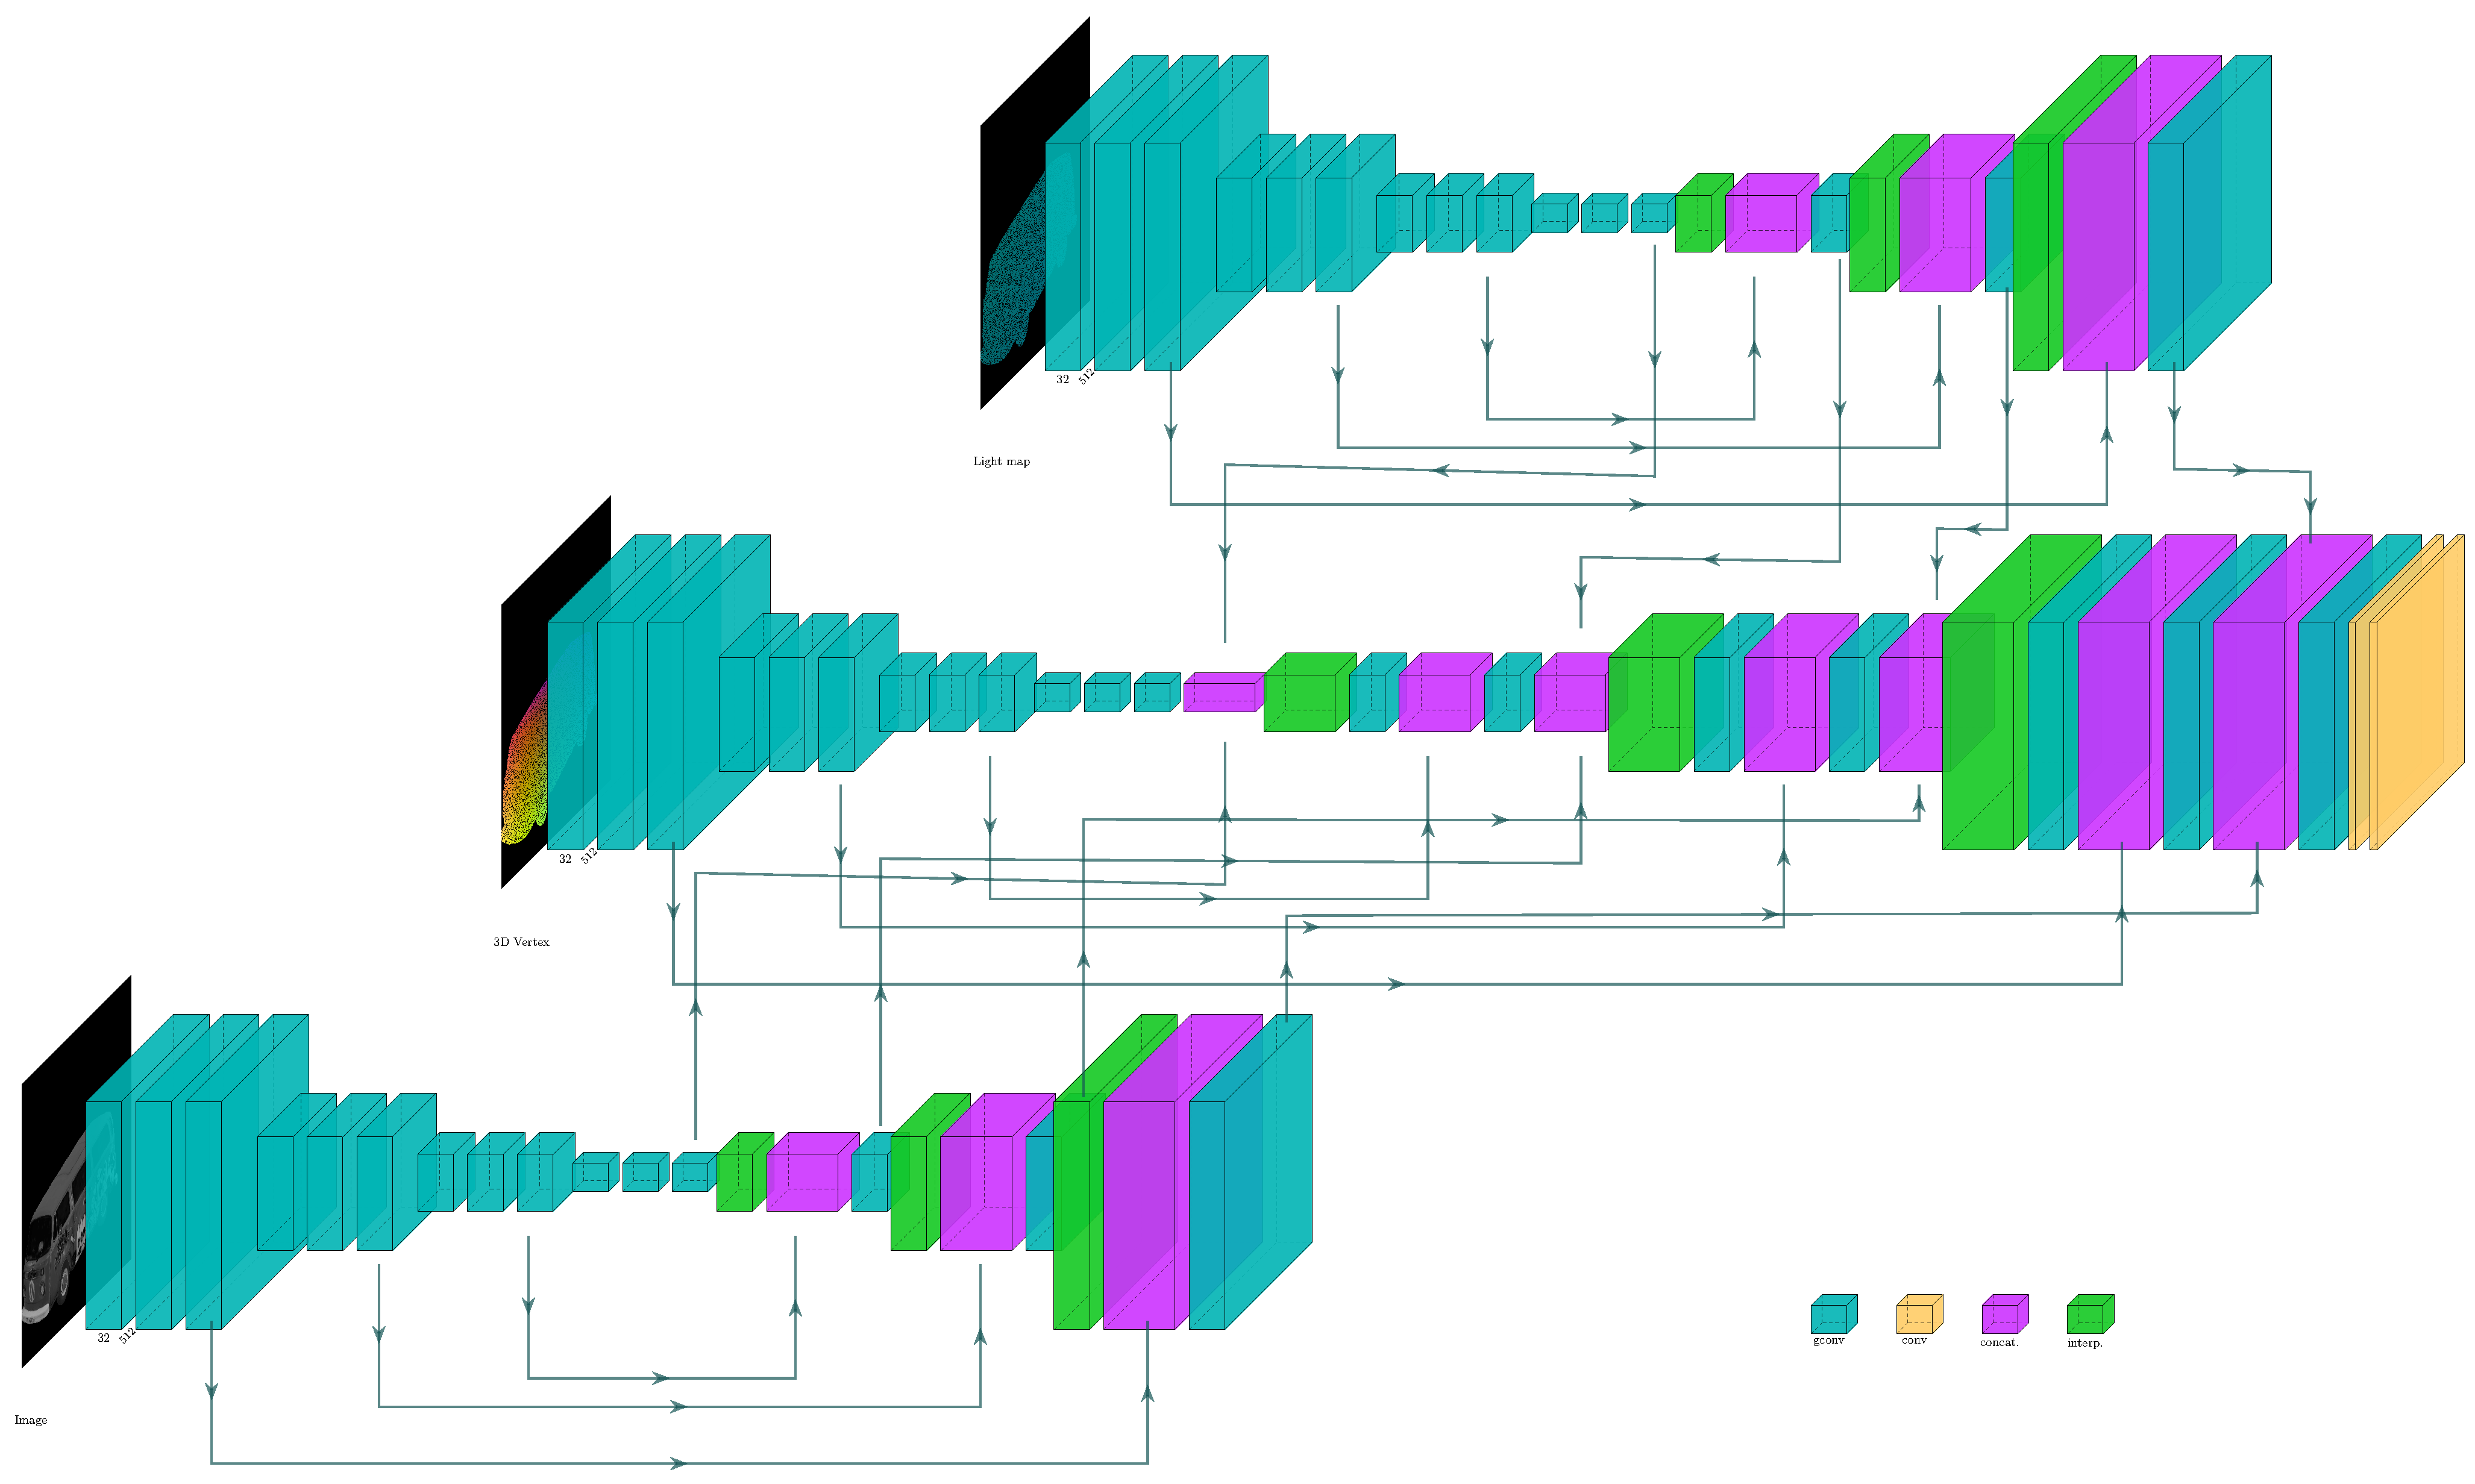
\includegraphics[width=1\textwidth]{Figures/trignet} % Research group name and department name
	\caption{The architecture of TriGNet}
	\label{fig:albedo-gated-archi}
\end{sidewaysfigure}


\subsection{Loss Function}
For the case of normal output, the loss function is the same as Mask-L2 loss as introduced in \ref{par:maskl2}. For the case of the product of albedo and normal, the loss function utilized a scaled Mask-L2 loss, which gives the range of inliers between $ [0,255] $. 




